\chapter{Traffic Monitoring}
\label{chap:trafficMonitoring}

A very important part of the thesis was to monitor the Wi-Fi traffic. Also, it was a prerequisite for all the following parts. Therefore, in this chapter, we also explain some facts that might be expected in the design section. We define hardware and software used for traffic monitoring along with the environment where we monitored the traffic. It is an important variable that influences Wi-Fi performance. At the end of the chapter, we will sum up all characteristics found based on both theoretical studies of the attack and practical traffic monitoring. We will refer to these conclusions and definitions in the following chapters.

\section{Prerequisites}
To be able to analyze the traffic in the Wi-Fi network, we need to be able to set our Wireless Interface Card (WNIC) into monitor mode. Ideally, we want to find a way how to cover the whole spectrum of channels in a band.

\subsection{Monitor Mode}
The monitor mode allows watching all Wi-Fi traffic on a specific channel without associating to an access point~\cite{captureSetupWireshark}. This mode is necessary to monitor 802.11 layer management and control frames. Also, the data frames would be encapsulated into a "fake" Ethernet packets. This layer is added by a wireless card driver~\cite{captureSetupWireshark}. Some commonly available wireless network cards can be switched to the monitor mode, but it is only possible with an appropriate driver. The availability of the driver depends on the combination of the OS and the chipset of the wireless card. The monitor mode does not change other characteristics of the card. Hence, with one card, it is possible to reliably capture traffic only on one channel at a time \cite{captureSetupWireshark}. 

\subsection{Hardware and Software}
\label{sub:hwAndsw}
As it has been mentioned, it is necessary to plug in the Wi-Fi card and control it by driver compatible with the OS. All current operating systems have support for wireless networks including tools and interfaces for network adapter control. For this work, we predominantly used Kali Linux operating system. Excellent overview of the options with other operating systems is available in~\cite{captureSetupWireshark} and \cite{Samek_2017}.

The availability of the drivers depends on the chipset of the wireless network card. Appropriate chipsets for Kali Linux are Atheros AR9271, Ralink RT3070, Ralink RT3572, Realtek 8187L, and Realtek RTL8812AU. If the built-in wireless network card does not have any of these chipsets, it is possible to use some Wi-Fi USB adapter. According to a few community bloggers, an Atheros AR9271 chipset is a decent choice for Kali Linux \cite{wirelesshack_2018, kaliChipsetDrivers_2018}. Hence, chose to use devices with this chipset. Very widespread used adapter with this chipset is the TP-LINK TL-WN722N v1. Unfortunately, other versions of this adapter (v2 and v3) have different chipsets, and the first version is not available anymore. Thus, we decided to use several Alfa AWUS036NHA adapters. The driver for this chipset is available in the kernel of the Kali Linux; and it is called \texttt{ath9k\_htc}. There are many command line tools that can be used for control of the wireless adapter, some of them are \texttt{airmon-ng}, \texttt{iw}, \texttt{iwconfig} and \texttt{iwlist}. 
To see the captured traffic, we can use programs \texttt{wireshark}, \texttt{tshark}, and \texttt{tcpdump}. All of them use the \texttt{libpcap} library. 

\subsection{Monitoring Multiple Channels}
The KRACK attack is targeted against both --- an AP and a client. Although we decided to focus on the attack on the 4-way handshake, we aimed to design such a tool that can be later extended by detection of other attacks of the family. Therefore, the system has to be independent of other devices in the network. It means that it has to be able to monitor the whole spectrum of channels. 
The Wi-Fi card can monitor on more channels by the so-called channel switching mechanism. It means it switches periodically between different channels. This mechanism is usually used for detecting the amount of traffic on different channels to find the least busy one~\cite{nirsoft_2014, tamosoft, levshova_2015, netspotapp_software_2019}. It is used to set the AP to a channel with the least interference and so, increase the speed of the connection. We need to monitor the channel for the whole time a handshake is in progress. Thus, this mechanism is not convenient for our solution. It implicates that the amount of channels we cover with our solution depends on the amount of Wi-Fi cards we will use. Also, we find out, it is a good practice to keep a distance at least 1 meter between interfaces monitoring on different channels. Otherwise, it might interfere with each other.

\section{Environment}
In this section, we are going to specify the environment in which we were monitoring the traffic. The traffic was monitored in two different environments with a different level of interference.

\begin{enumerate}[I.]
\label{enum:environments}
    \item On campus, building A, i.e., many Wi-Fi devices, very high interference. Data measured during the semester, during the day.
    \item \label{env:B} A house with more housing units, four flours, second floor, two-room apartment, data measured during the day, less interference.
\end{enumerate}

\begin{figure}[h!]
  \centering
  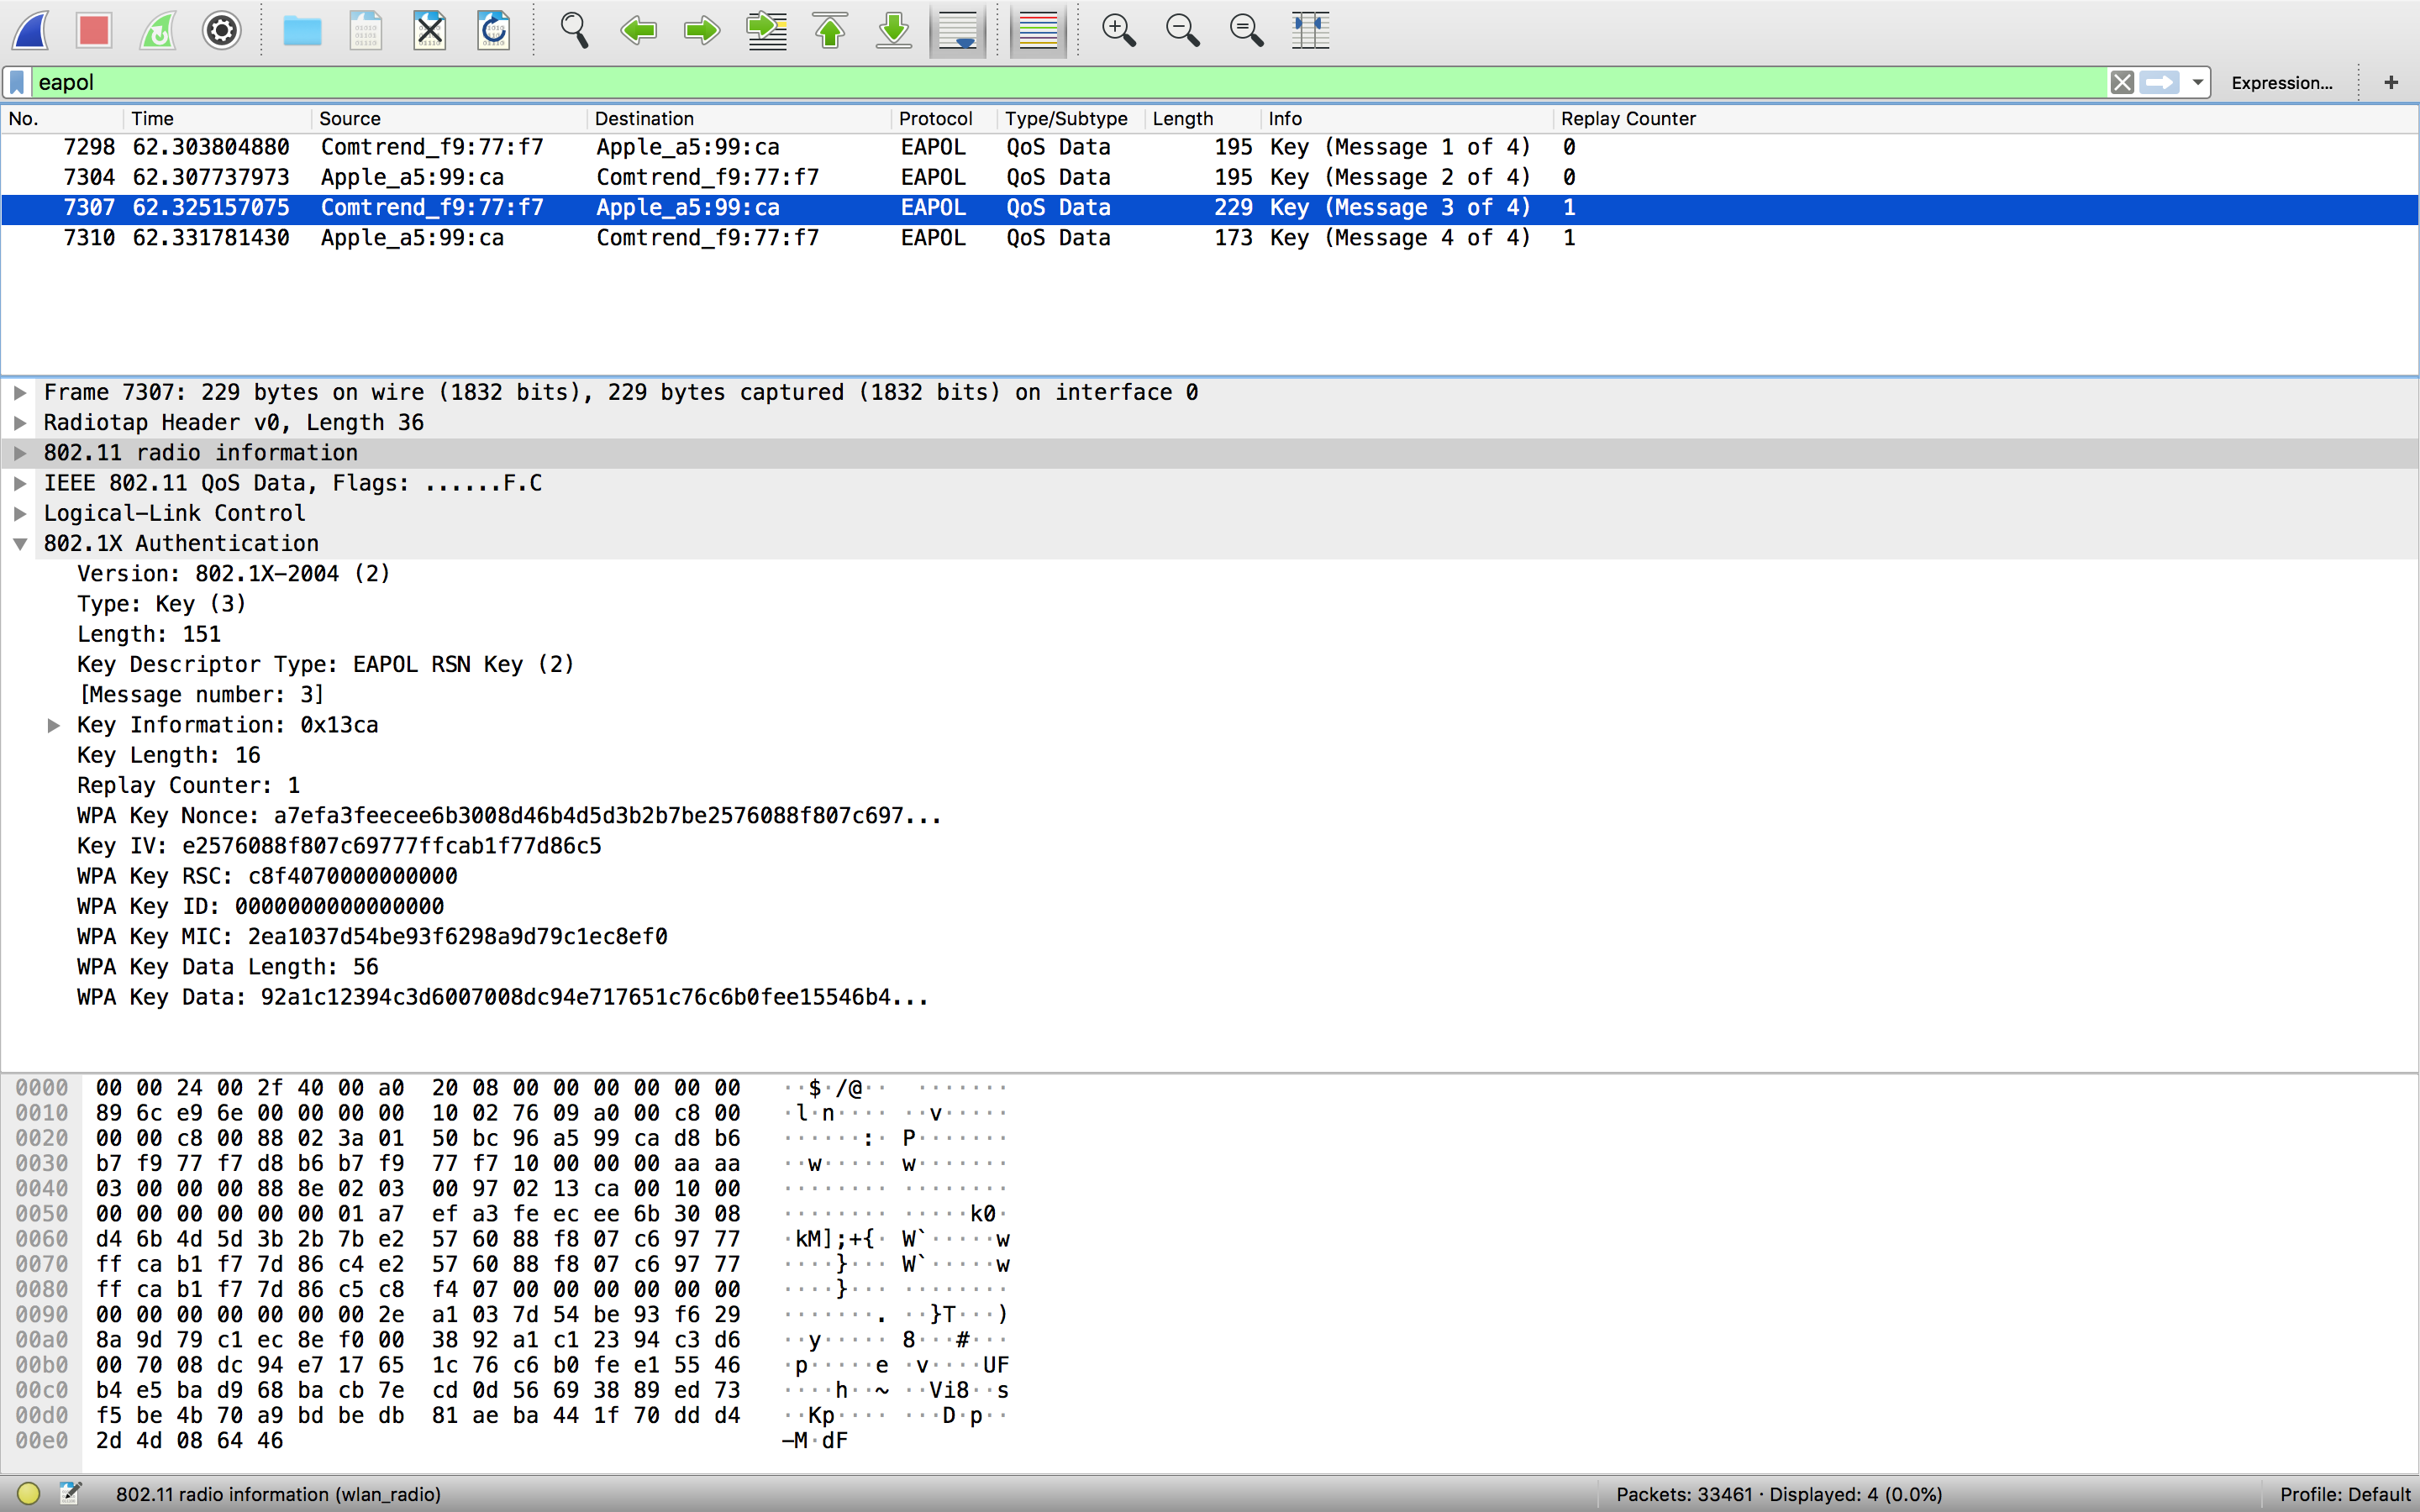
\includegraphics[scale=0.4, angle=90]{img/4_way_handshake.png}
  \caption[The 4-way handshake captured in wireshark]{The 4-way handshake captured in wireshark.}
  \label{fig:4wayHandshake}
\end{figure}

\section{Standard 4-way Handshake}
\label{sec:standardFourWayHandshake}

First, the standard traffic of the 4-way handshake was monitored. In Figure~\ref{fig:4wayHandshake}, there is an example of the captured 4-way handshake in program wireshark. This handshake was captured without any anomalies. We filtered it from other captured traffic by using \texttt{eapol} filter. In this specific example, there was no other handshake captured. Thus, no additional filtering was necessary. The type of the frame is QoS Data and used protocol is EAPOL. In the Info field, we can see the order of the messages. Wireshark identified the number of each message by used flags in Key Description field and by information contained in the frame. We will also need to watch field Replay counter, as explained in Section~\ref{sec:attackPrinciple} and WPA Key Nonce which will help us uniquely identify each 4-way handshake between the same pair of devices. Also, we can see in the Address fields Source and Destination, that this handshake took place between the AP (MAC address \texttt{Comtrend\_f9:77:f7}) and the client (\texttt{Apple\_a5:99:ca}). Below the list of frames, we can see details of the \textit{message~3} of the handshake. Specifically, the 802.1x layer, which is expanded, contains the WPA Key Nonce. Below, we can see the raw payload that was parsed by wireshark to get all this information.

The 4-way handshake shown in Section~\ref{fig:4wayHandshake} is perfectly corresponding to the standard, but during the analysis of the traffic, two anomalies were often detected. It often happened that one of the messages of the handshake was lost due to interference. Indeed, in the network on campus. The other detected non-standard behavior is often immediate repetition of \textit{message~1} of the 4-way handshake. Thus, these sequences of messages will be considered normal, non-malicious behavior.

\section{Malicious 4-way Handshake}
\label{sec:maliciousTraffic}

For the study of the traffic generated during the attack, we used scripts~\cite{vanhoefm_2018} that author published as a proof-of-concept. It was necessary to modify them to be able to successfully perform the attack. Also, we studied publicly available scripts~\cite{vanhoefm_2018} made for detecting a device vulnerability to this attack. There is a \textit{.pcap} file captured during the attack in Figure~\ref{fig:krackAttackTraffic}. We filtered the pair of the AP and the client performing the handshake. For the sake of clarity, we have filtered out Action and Null function frames. Note, that you can see there is the same ANonce in all messages 1 and 3 in the figure. This means it is still the same handshake and the same PTK is negotiated. During monitoring of the attack traffic, we found several often or always occurring characteristics:

\begin{description}
\item \textbf{Retransmitted message 3}: The most important characteristics of the attack is retransmitted \textit{message~3} of the handshake. We can see the frame with No.~1954 in Figure~\ref{fig:krackAttackTraffic}. In case this happens, we should evaluate the situation as a possible KRACK attack in the network. 
\item \textbf{Repeated message 1 after message 3}: The attacker sometimes tries to abuse the vulnerability of the supplicant by sending \textit{message~1} before retransmitting \textit{message~3}. We can see this as frame No.~1952 in Figure~\ref{fig:krackAttackTraffic}. This vulnerability corresponds to the state machine of the vulnerable supplicant in Figure~\ref{fig:stateMachineSupplicant}. Also, Vanhoef states~\cite{VA_ccs2017} that it is a necessary step when attacking specific devices. However, this characteristics does not mean the attack is completed.
\item \textbf{Reset of the packet number after retransmitted message~3}: This is the main point of the attack. If we can capture this, this means the frames can be decrypted, either it happened due to the interference, or it was triggered by an attacker. We can see this in Figure~\ref{fig:krackAttackTraffic} as frames No.~1964 and No.~1973. They both use the same packet number, in this case, the CCMP encryption algorithm is used, so the packet number corresponds to CCMP Ext. Intialization Vector. We are not always able to capture the first data frame to confirm the hypothesis.
\item \textbf{Very high occurrence of message 3}: Monitoring traffic during the attack, it was found that there is a much higher occurrence of the \textit{message~3} of the handshake in the traffic. We can see this in Figure~\ref{fig:krackAttackTraffic} as frames No.~1146, 1147, 1226, 1227, 1311, 1312. Even though they do not have to lead to a successful exploit of the vulnerability, their occurrence very likely means the presence of an attacker in the network or very high interference of the environment. We can distinguish between them by counting ration of captured \textit{messages~1} to \textit{messages~3} in the same handshake. As we stated in \ref{sec:standardFourWayHandshake}, the repetition of \textit{message~1} is a standard behavior. Thus, when there are significantly more messages 3 then messages 1 of the handshake, it is likely that an attacker is trying to exploit this vulnerability.
\item \textbf{Frequent failure of the handshake}: Another characteristic that can make us suspicious is the number of handshakes that fail. When the attacker is performing the attack, there are many handshakes that are triggered again during the handshake. Thus, they fail. 
\end{description}

\section{Characteristics For Detection}
This section provides a summary of all found characteristics we could use for detection of the KRACK attack against the 4-way handshake.

\subsection{Based on the Analysis of the Captured Traffic}
Based on Section~\ref{sec:standardFourWayHandshake} and Section~\ref{sec:maliciousTraffic}, we found several characteristics for the detection. There are two points of view of how to look at it. The first one is by searching concrete sequences of messages of the handshake. The second is by establishing characteristics either for the environment in general or for each handshake by using statistical methods.

\subsubsection*{Concrete Sequence of Messages}
We can look at the concrete sequence of messages that we see in both malicious and standard communication and create a state machine that would have an acceptance state in case the attack was performed.

\subsubsection*{General Characteristics of the Environment}
Another option would be to create a statistical model of the situation. Based on the monitored traffic, we can create a model of a standard handshake with all the anomalies found in normal communication. Then, we can detect anomalies against it. Good characteristics to use in such a model would be the frequency of each message of the handshake (e.g., a high occurrence of \textit{message~3} in the communication). To use it, we would have to find a threshold, which can significantly differ in networks with different level of interference. It would not be as reliable as a concrete sequence of messages.

\subsection{Based on Theoretical Study of the Attack}
The detection would also be possible by characteristics found in the theoretical description of the attack. 

One option available for detection of the attack against the 4-way handshake is detecting the channel based MitM position. In the research which introduced this attack in 2014~\cite{Va_2014}, the author states, the attack could be detected on the client side, by including the channel of the AP in the 4-way handshake. Unfortunately, this would require a change of the protocol itself because the channel is not included in the frame. Interesting question for future research is if the detection of channel based MitM would be possible with monitoring devices on multiple channels. But it is beyond the scope of this work. There are some products in the market dealing with detection of MitM in the Wi-Fi network, for example, ~\cite{zimperium_2018}.

According to the vulnerabilities found following characteristics should be exactly what leads to a successful exploit. Since the Wi-Fi network is very prone to the interference, some of the messages can be lost even if it is successfully transmitted between the attacker and the victim. Thus, when using only these characteristics, some attacks might be missed completely.

\begin{description}
\item \textbf{the 4-way handshake}: Retransmitted \textit{message~3} of the 4-way handshake with incremented replay counter. Then, the client will receive \textit{message~3} multiple times and because of the increased replay counter, he or she should accept it. If the next sent data frame from the client to the AP has lower packet number than the previous packets, the packet number was reset, and so the PTK reinstalled. 
\item \textbf{the PeerKey handshake}: The 4-way handshake used in the second phase of the PeerKey handshake is attacked in the same manner. Thus, for detection this attack, we can use the same techniques as for detection of the attack to the 4-way handshake. The difference is only in used flags which identify used keys and the handshake.
\item \textbf{Group key handshake}: Retransmitted \textit{message~3} of the group key handshake from AP and reinitializing of the replay counter of the GTK at the client side. 
\item \textbf{The Fast BSS Transition Handshake (FT) Handshake}: This is the only attack against the AP. Looking for retransmitted Reassociation request which serves as \textit{message~3} of the FT handshake. Following reset of the packet number and replay counter in next sent data frame means certain to exploit.
\item \textbf{Fast Initial Link Setup handshake}: Again, we can look for replayed (Re)Association requests and following reinstallation of the PTK and re-usage of packet number.
\item \textbf{TDLS PeerKey handshake}: In case of this handshake, we need to detect retransmitted TDLS Setup Response frame and following reuse of packet number after completion of the handshake.
\item \textbf{WNM-Sleep response frames}: These frames can be abused to trigger key reinstallations. It would be a good practice to detect retransmitted WNM-Sleep exit frames to avoid it. How these Null frames are used to trigger key reinstallation is further explained in \cite{VA_ccs2018}.
\end{description}

\begin{figure}[h!]
  \centering
  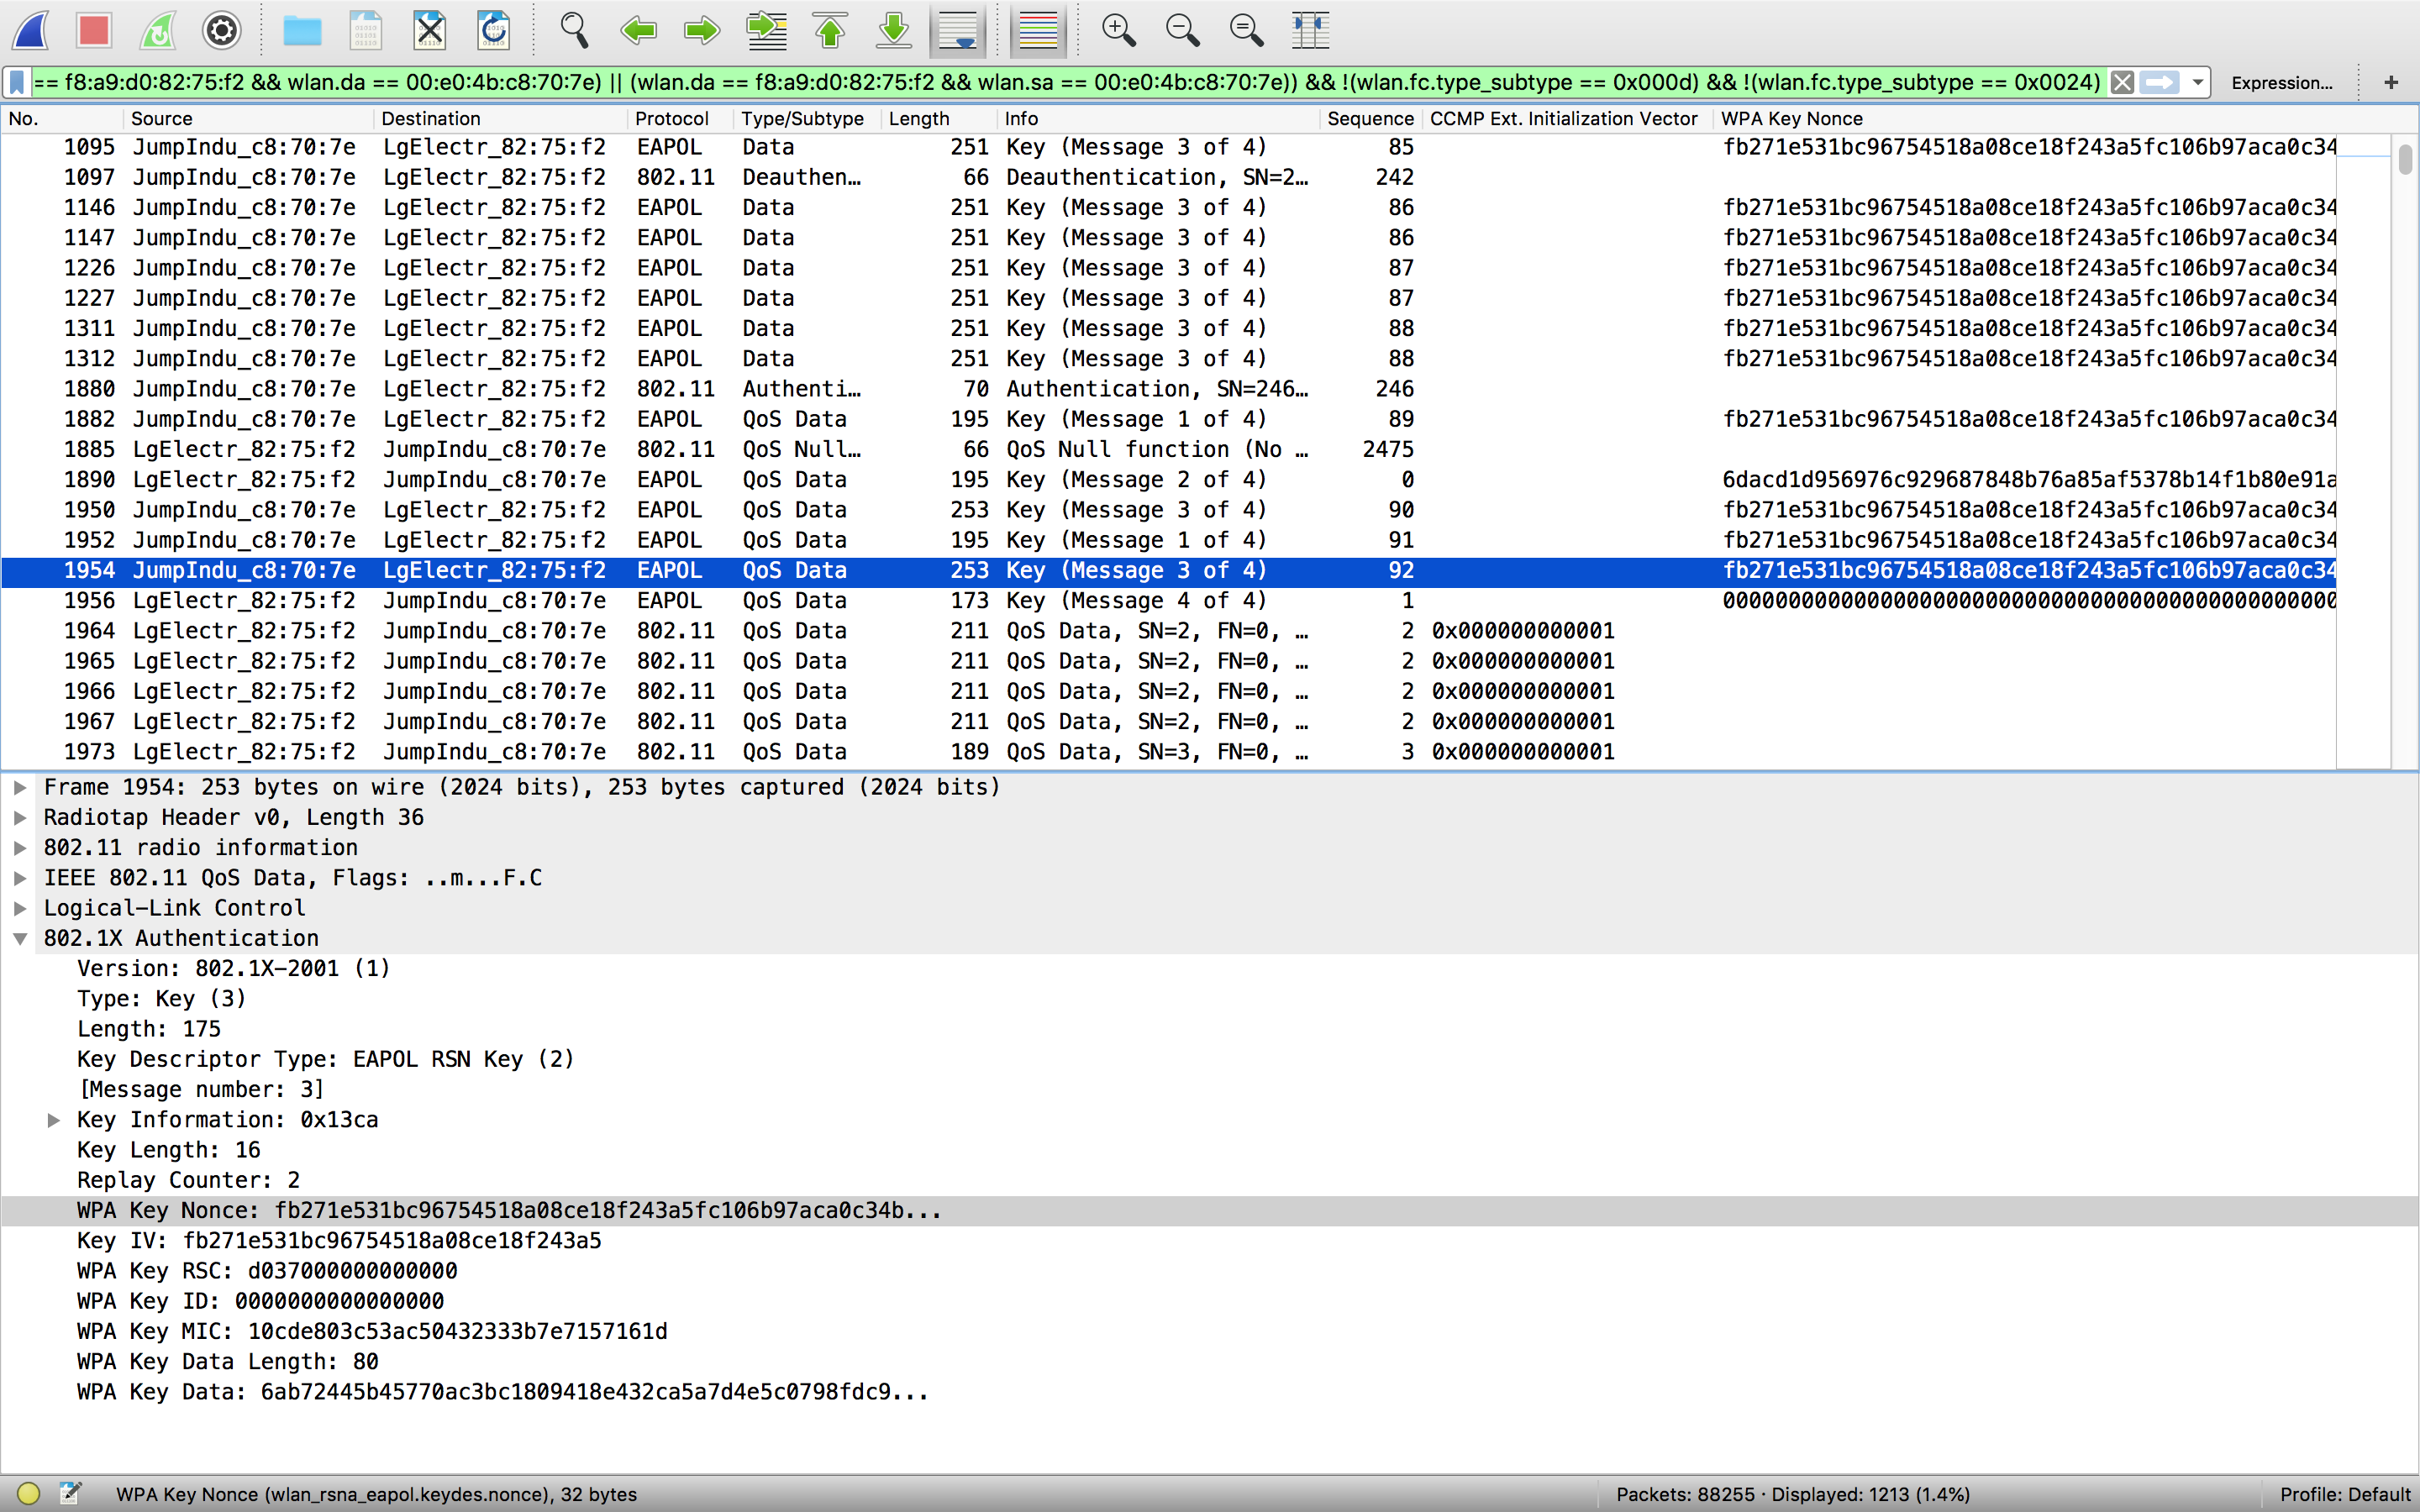
\includegraphics[scale=0.37, angle=90]{img/attackPcap.png}
  \caption[Traffic generated by successful KRACK attack against the 4-way hanshake]{Traffic generated by successful KRACK attack against the 4-way hanshake.}
  \label{fig:krackAttackTraffic}
\end{figure}